\section{Management Summary}
\subsection*{Ausgangslage}
OpenStreetMap, eine online Kartenanwendung wie Google Maps, bietet Daten, die für Fussgängernavigation genutzt werden können. Dabei müssen die bestehenden Fussgängerstreifen in die Planung einbezogen werden, um eine Überquerung der Strassen zu ermöglichen. Unglücklicherweise sind nicht alle Fussgängerstreifen in OpenStreetMap erfasst, was die Fussgängernavigation erschwert.

Dieses Projekt ist der Versuch einer automatischen Erkennung von Fussgängerstreifen auf Orthofotos (umgangssprachlich Satellitenbilder). Da das maschinelle Erfassen von Daten in OpenStreetMap nicht erlaubt ist, müssen die gefundenen Koordinaten in ein Crowdsourcing-System wie MapRoulette eingespeist werden. In diesem bewerten Nutzer, ob die eingefügten Daten korrekt sind oder nicht.

\subsection*{Vorgehen}
\begin{figure}[H]
	\centering
	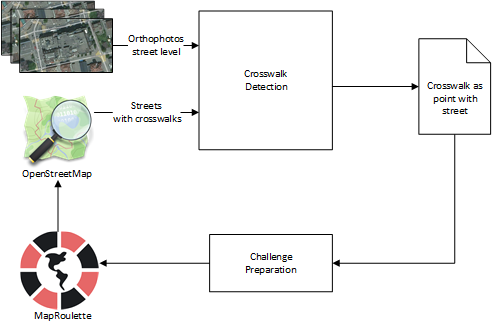
\includegraphics[width=410pt]{images/management_summary_1.png}
	\caption[Management Summery Überblick]{Überblick}
\end{figure}
Wir begannen die Arbeit mit der Evaluation eines passenden Bilderkennungsalgorithmus. Dabei haben wir diverse Algorithmen vom Haar Feature-based Cascade Classifier über Fast Fourier Transform bis zu Neuronalen Netzen implementiert und getestet. Ein neuronales Netz, genauer ein Convolutional Neural Network, brachte die besten Resultate bei der Klassifikation der Bilder.

Weiter mussten Orthofotos, wie auch Informationen zu Strassenverläufe und die Koordinaten der schon erfassten Fussgängerstreifen beschafft werden. Dabei konnte auf Bing Maps und die Programmierschnittstelle von Mapquest zurückgegriffen werden.

Da die Bilderkennung ein sehr rechenintensiver Prozess ist, mussten wir den Erkennungsprozess parallelisieren. Mithilfe eines Docker Images und einem Queueing System konnte die Erkennung auf verschiedene Maschinen verteilt und der Erkennungsaufwand auf mehrere Tage beschränkt werden. Ohne diese Parallelisierung hätten Wartezeiten von mehreren Wochen in Kauf genommen werden müssen.


\subsection*{Ergebnisse}
Aus diesem Projekt entstand einen Applikation für die automatische Erkennung von Fussgängerstreifen. Diese bezieht in einem angegebenen Bereich, wie beschrieben, automatisch die entsprechenden Orthofotos und Strasseninformationen und extrahiert daraus die Koordinaten der Fussgängerstreifen. Die Koordinaten werden in einer JSON-Datei abgelegt und können in eine MapRoulette Challenge umgewandelt werden. 
\\
\begin{figure}[H]
	\centering
	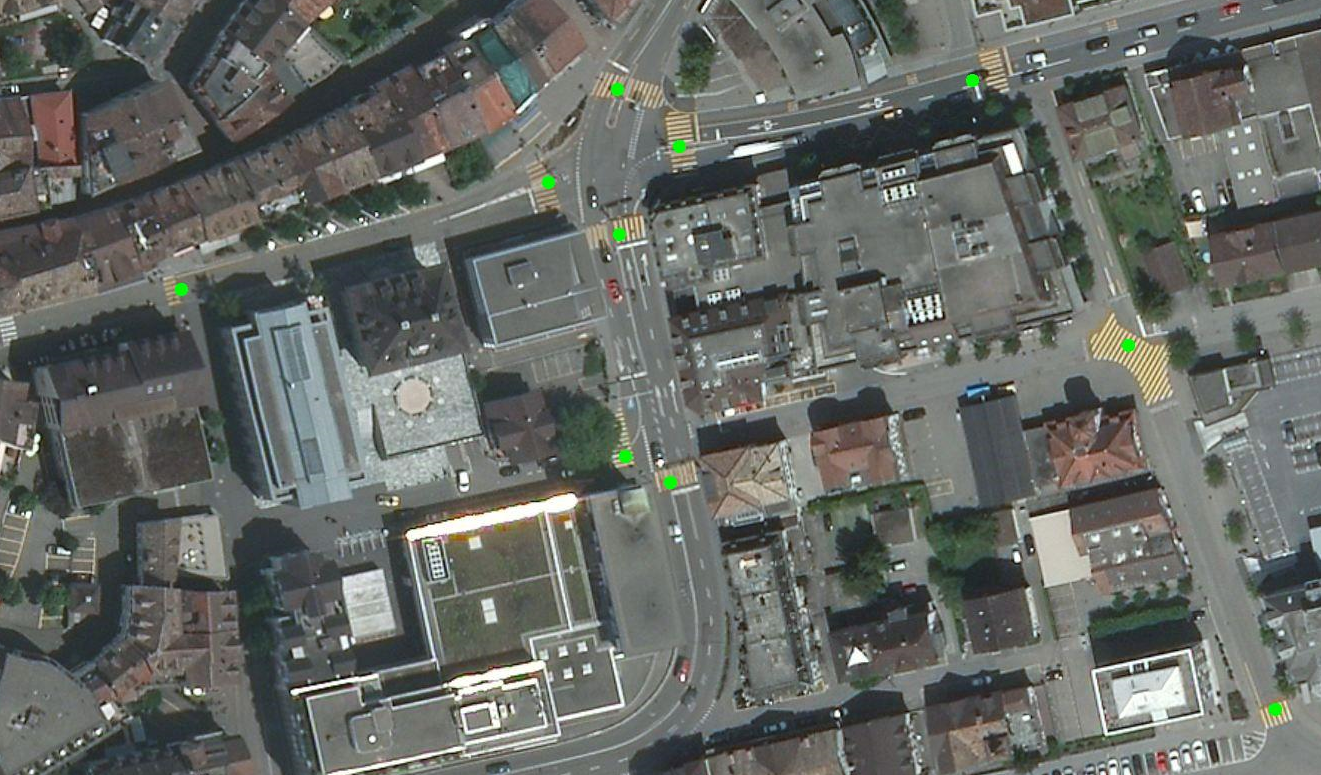
\includegraphics[width=\textwidth -10mm]{images/boxsave_rappi.png}
	\caption[Überblick]{Rapperswil Innenstadt - Gefundene Fussgängerstreifen sind mit einem grünen Punkt markiert.}
\end{figure}

Die Applikation erkannte mehr als 80\% aller gelben Fussgängerstreifen mit einer Fehlerrate von weniger als 10\%. Die Koordinaten der Fussgängerstreifen im Raum der Kantone Zürich und Zug konnten an MapRoulette zur Einpflegung in OpenStreetMap übergeben werden.
\\
\begin{figure}[H]
	\centering
	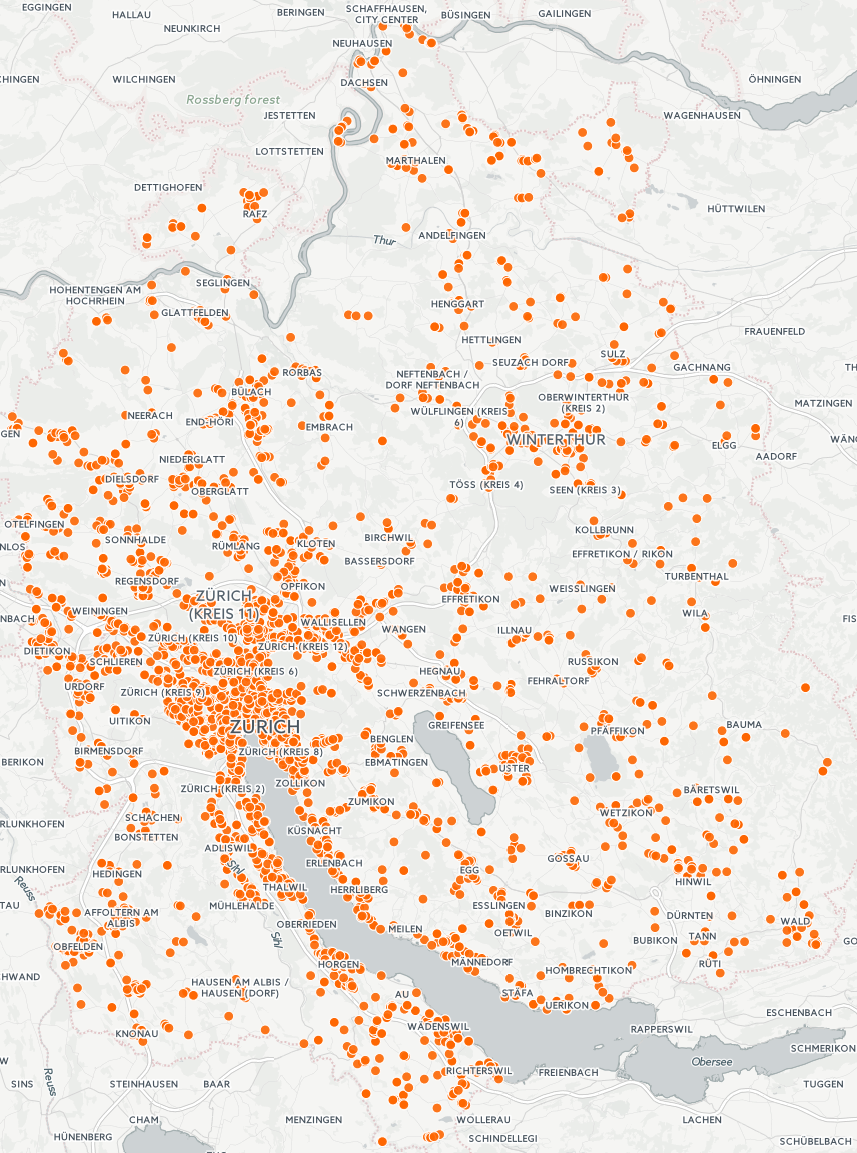
\includegraphics[width=\textwidth -80mm]{images/karte.png}
	\caption{Gesamtresultat Zürich}
\end{figure}

\subsection*{Ausblick}
Der Erkennungsalgorithmus ist zu Ende dieses Projektes auf die Region Zürich und die Ostschweiz spezialisiert. Mit weiteren Optimierungen beim Neuronalen Netz ist es möglich, alle Fussgängerstreifen in der Schweiz zu erfassen und sogar weisse Fussgängerstreifen für andere europäische Länder zu erkennen. Auch weitere Strassenmarkierungen sind denkbar.

Weiter ist die Geschwindigkeit, in der Convolutional Neural Network verbessert werden, enorm. In 2 - 3 Jahren könnte es möglich sein, annähernd alle Fussgängerstreifen auf Orthofotos zu erkennen.
\newpage